Observing that $\Ub_1\kron\Ub_2\kron\Ub_3$ is a left-orthogonal matrix, it follows that 
 $\norm{\Tt} = \norm{\vectorize(\Tt)} = \norm{(\Ub_1\kron\Ub_2\kron\Ub_3)\vectorize(\Tt)}= \norm{\vectorize(\Gt)} = \norm{\Gt}$.
    


    \item If we do not enforce any orthogonality constraints on the factor matrices and fix the core tensor to be a copy tensor,
$
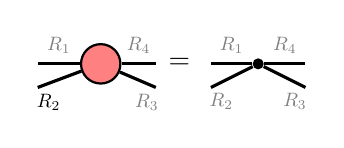
\begin{tikzpicture}[baseline=-0.5ex]
    \tikzset{tensor/.style = {minimum size = 0.5cm,shape = circle,thick,draw=black,inner sep = 0pt}, edge/.style = {thick,line width=.4mm},every loop/.style={}}
    \def\x{6}
    \def\y{0}
    \node[tensor,fill=red!50!white] (G) at (\x+4.5,\y) {$\Gt$};
    \draw[edge] (G) -- (\x+5.2,\y) node [midway, above] {\scalebox{0.7}{\textcolor{gray}{$R_4$}}};
    \draw[edge] (G) -- (\x+3.7,\y-0.3) node [below, near end] {\scalebox{0.7}{\dimcolor{$R_2$}}};
    \draw[edge] (G) -- (\x+5.2,\y-0.3) node [below, near end] {\scalebox{0.7}{\textcolor{gray}{$R_3$}}};
    \draw[edge] (G) -- (\x+3.7,\y) node [midway, above] {\scalebox{0.7}{\textcolor{gray}{$R_1$}}};
    \node[draw = none] at (\x+5.5,0){$=$};
    \draw  node[fill = black,circle,inner sep=0pt,minimum size=4pt] (m) at (\x+6.5,\y) {};
    \draw[edge] (m) -- (\x+7.1,\y) node [midway, above] {\scalebox{0.7}{\textcolor{gray}{$R_4$}}};
    \draw[edge] (m) -- (\x+5.9,\y-0.3) node [below, near end] {\scalebox{0.7}{\textcolor{gray}{$R_2$}}};
    \draw[edge] (m) -- (\x+7.1,\y-0.3) node [below, near end] {\scalebox{0.7}{\textcolor{gray}{$R_3$}}};
    \draw[edge] (m) -- (\x+5.9,\y) node [midway, above] {\scalebox{0.7}{\textcolor{gray}{$R_1$}}};
\end{tikzpicture},
$
we recover the CP decomposition. %
    \item \label{item:Tucker_orth} If $\Tt = \Gt\ttm{1}\Ab_1\ttm{2}\Ab_2\ttm{3}\Ab_3\ttm{4}\Ab_4$, with $\Ab_1,\Ab_2,\Ab_3$ and $\Ab_4$ not necessarily orthogonal, then there exists $\Tilde{\Gt}$ (of the same size as $\Gt$) and $\Qb_1,\Qb_2,\Qb_3$ and $\Qb_4$ orthogonal such that $\Tt = \Tilde{\Gt}\ttm{1}\Qb_1\ttm{2}\Qb_2\ttm{3}\Qb_3\ttm{4}\Qb_4$.
    \begin{proof}
By performing QR decomposition on each factor matrix, we obtain
\begin{align*}
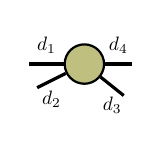
\begin{tikzpicture}[baseline=-0.5ex]
    \tikzset{tensor/.style = {minimum size = 0.5cm,shape = circle,thick,draw=black,inner sep = 0pt}, edge/.style = {thick,line width=.4mm},every loop/.style={}}
    \def\x{6}
    \def\y{0}   \node[tensor,fill=green!50!red!50!white] (T) at (\x+1,\y) {$\Tt$};
    \draw[edge] (T) -- (\x+0.3,0) node [midway,above] {\scalebox{0.7}{\dimcolor{$d_1$}}};
    \draw[edge] (T) -- (\x+1.6,0) node [midway,above] {\scalebox{0.7}{\dimcolor{$d_4$}}};;
    \draw[edge] (T) -- (\x+0.4,-0.3) node [midway, below] {\scalebox{0.7}{\dimcolor{$d_2$}}};
    \draw[edge] (T) -- (\x+1.5,-0.4)node [midway, below] {\scalebox{0.7}{\dimcolor{$d_3$}}};
\end{tikzpicture}
&=
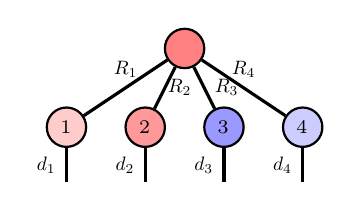
\begin{tikzpicture}[baseline=-0.5ex]
    \tikzset{tensor/.style = {minimum size = 0.5cm,shape = circle,thick,draw=black,inner sep = 0pt}, edge/.style = {thick,line width=.4mm},every loop/.style={}}
    \def\x{6}
    \def\y{0}   
    \node[tensor,fill=red!50!white] (G) at (\x+4.5,\y+1) {$\Gt$};
    \node[tensor,fill=red!20!white] (A_1) at (\x+3,\y){$\Ab_1$};
    \node[tensor,fill=red!40!white] (A_2) at (\x+4,\y){$\Ab_2$};
    \node[tensor, fill=blue!40!white] (A_3) at (\x+5,\y){$\Ab_3$};
    \node[tensor,fill=blue!20!white] (A_4) at (\x+6,\y){$\Ab_4$};
    \draw[edge] (G) -- (A_1) node [midway, above] {\scalebox{0.7}{\dimcolor{$R_1$}}};
    \draw[edge] (G) -- (A_2) node [midway, right=-0.1cm] {\scalebox{0.7}{\dimcolor{$R_2$}}};
    \draw[edge] (G) -- (A_3) node [midway, right=-0.05] {\scalebox{0.7}{\dimcolor{$R_3$}}};
    \draw[edge] (G) -- (A_4) node [midway, above] {\scalebox{0.7}{\dimcolor{$R_4$}}};
    \draw[edge] (A_1) -- (\x+3,\y-0.7) node [midway, left] {\scalebox{0.7}{\dimcolor{$d_1$}}};
    \draw[edge] (A_2) -- (\x+4,\y-0.7) node [midway, left] {\scalebox{0.7}{\dimcolor{$d_2$}}};
    \draw[edge] (A_3) -- (\x+5,\y-0.7) node [midway, left] {\scalebox{0.7}{\dimcolor{$d_3$}}};
    \draw[edge] (A_4) -- (\x+6,\y-0.7) node [midway, left] {\scalebox{0.7}{\dimcolor{$d_4$}}};
\end{tikzpicture}\\
&=
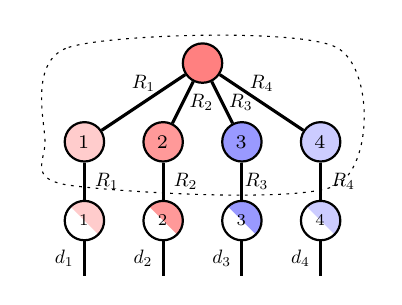
\begin{tikzpicture}[baseline=-0.5ex]
    \tikzset{tensor/.style = {minimum size = 0.5cm,shape = circle,thick,draw=black,inner sep = 0pt}, edge/.style = {thick,line width=.4mm},every loop/.style={}}
    \def\x{6}
    \def\y{0}   
   \node[tensor,fill=red!50!white] (G) at (\x+9,\y+1) {$\Gt$};
    \node[tensor,fill=red!20!white] (R_1) at (\x+7.5,\y){$\Rb_1$};
    \node[tensor,fill=red!40!white] (R_2) at (\x+8.5,\y){$\Rb_2$};
    \node[tensor, fill=blue!40!white] (R_3) at (\x+9.5,\y){$\Rb_3$};
    \node[tensor,fill=blue!20!white] (R_4) at (\x+10.5,\y){$\Rb_4$};
    \node[tensor, path picture={
    \fill[fill=red!20!white](path picture bounding box.south east)
    -- 
    (path picture bounding box.north west) --
    (path picture bounding box.north east) -- cycle;
    }, shift={(\x+7.5,\y-1)}] (Q_1)  {\scalebox{0.85}{$\Qb_1$}};  \node[tensor, path picture={
    \fill[fill=red!40!white](path picture bounding box.south east)
    -- 
    (path picture bounding box.north west) --
    (path picture bounding box.north east) -- cycle;
    }, shift={(\x+8.5,\y-1)}] (Q_2) {\scalebox{0.85}{$\Qb_2$}};
    \node[tensor, path picture={
    \fill[fill=blue!40!white](path picture bounding box.south east)
    -- 
    (path picture bounding box.north west) --
    (path picture bounding box.north east) -- cycle;
    }, shift={(\x+9.5,\y-1)}] (Q_3) {\scalebox{0.85}{$\Qb_3$}};
        \node[tensor, path picture={
    \fill[fill=blue!20!white](path picture bounding box.south east)
    -- 
    (path picture bounding box.north west) --
    (path picture bounding box.north east) -- cycle;
    }, shift={(\x+10.5,\y-1)}] (Q_4) {\scalebox{0.85}{$\Qb_4$}};
    \draw[edge] (G) -- (R_1) node [midway, above] {\scalebox{0.7}{\dimcolor{$R_1$}}};
    \draw[edge] (G) -- (R_2) node [midway, right=-0.05cm] {\scalebox{0.7}{\dimcolor{$R_2$}}};
    \draw[edge] (G) -- (R_3) node [midway, right=-0.05cm] {\scalebox{0.7}{\dimcolor{$R_3$}}};
    \draw[edge] (G) -- (R_4) node [midway, above] {\scalebox{0.7}{\dimcolor{$R_4$}}};
    \draw[edge] (R_1) -- (Q_1) node [midway, right] {\scalebox{0.7}{\dimcolor{$R_1$}}};
    \draw[edge] (R_2) -- (Q_2) node [midway, right] {\scalebox{0.7}{\dimcolor{$R_2$}}};
    \draw[edge] (R_3) -- (Q_3) node [midway, right=-0.1cm] {\scalebox{0.7}{\dimcolor{$R_3$}}};
    \draw[edge] (R_4) -- (Q_4) node [midway, right] {\scalebox{0.7}{\dimcolor{$R_4$}}};
    \draw[edge] (Q_1) -- (\x+7.5,\y-1.7) node [midway, left] {\scalebox{0.7}{\dimcolor{$d_1$}}};
    \draw[edge] (Q_2) -- (\x+8.5,\y-1.7) node [midway, left] {\scalebox{0.7}{\dimcolor{$d_2$}}};
    \draw[edge] (Q_3) -- (\x+9.5,\y-1.7) node [midway, left] {\scalebox{0.7}{\dimcolor{$d_3$}}};
    \draw[edge] (Q_4) -- (\x+10.5,\y-1.7) node [midway, left] {\scalebox{0.7}{\dimcolor{$d_4$}}};
    \draw[dash pattern=on 1pt off 2pt] plot[smooth cycle] coordinates { 
    (\x+7,\y) 
    (\x+7.3, \y+1.2) (\x+10.7,\y+1.2) (\x+10.7, \y-0.55)  (\x+7.3,\y-0.55)};
\end{tikzpicture}
=
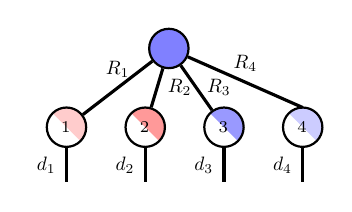
\begin{tikzpicture}[baseline=-0.5ex]
    \tikzset{tensor/.style = {minimum size = 0.5cm,shape = circle,thick,draw=black,inner sep = 0pt}, edge/.style = {thick,line width=.4mm},every loop/.style={}}
    \def\x{6}
    \def\y{0}   
    \node[tensor,fill=blue!50!white] (G) at (\x+13.5,\y+1) {$\Tilde{\Gt}$};
    \node[tensor, path picture={
    \fill[fill=red!20!white](path picture bounding box.south east)
    -- 
    (path picture bounding box.north west) --
    (path picture bounding box.north east) -- cycle;
    }, shift={(\x+12.2,\y)}] (Q_1)  {\scalebox{0.85}{$\Qb_1$}};  \node[tensor, path picture={
    \fill[fill=red!40!white](path picture bounding box.south east)
    -- 
    (path picture bounding box.north west) --
    (path picture bounding box.north east) -- cycle;
    }, shift={(\x+13.2,\y)}] (Q_2) {\scalebox{0.85}{$\Qb_2$}};
    \node[tensor, path picture={
    \fill[fill=blue!40!white](path picture bounding box.south east)
    -- 
    (path picture bounding box.north west) --
    (path picture bounding box.north east) -- cycle;
    }, shift={(\x+14.2,\y)}] (Q_3) {\scalebox{0.85}{$\Qb_3$}};
        \node[tensor, path picture={
    \fill[fill=blue!20!white](path picture bounding box.south east)
    -- 
    (path picture bounding box.north west) --
    (path picture bounding box.north east) -- cycle;
    }, shift={(\x+15.2,\y)}] (Q_4) {\scalebox{0.85}{$\Qb_4$}};
     \draw[edge] (Q_1) -- (\x+12.2,\y-0.7) node [midway, left] {\scalebox{0.7}{\dimcolor{$d_1$}}};
    \draw[edge] (Q_2) -- (\x+13.2,\y-0.7) node [midway, left] {\scalebox{0.7}{\dimcolor{$d_2$}}};
    \draw[edge] (Q_3) -- (\x+14.2,\y-0.7) node [midway, left] {\scalebox{0.7}{\dimcolor{$d_3$}}};
    \draw[edge] (Q_4) -- (\x+15.2,\y-0.7) node [midway, left] {\scalebox{0.7}{\dimcolor{$d_4$}}};
    \draw[edge](G) -- (Q_1)node[midway,above]{\scalebox{0.7}{\dimcolor{$R_1$}}};
    \draw[edge](G) -- (Q_2)node[midway,right]{\scalebox{0.7}{\dimcolor{$R_2$}}};
    \draw[edge](G) -- (Q_3)node[midway,right]{\scalebox{0.7}{\dimcolor{$R_3$}}};
    \draw[edge](G) -- (\x+15.2,\y+0.25)node[midway,above]{\scalebox{0.7}{\dimcolor{$R_4$}}};
\end{tikzpicture}.
\end{align*}
\end{proof}
\item For an $N$-th order $d$-dimensional tensor, the number of parameters in its Tucker decomposition is $\bigo(R^N+NdR)$ assuming $R_1=\dots=R_N=R$.
\item
We conclude this section by showing how the mode-$n$ matricization of the Tucker decomposition of a tensor can be expressed using Kronecker products.
\begin{proposition}\label{decomp:tucker-kron}
Let $\At\in\RR^{d_1\times d_2\times\dots\times d_N}$. If $\At=\Gt\ttm{1}\Ub_1\ttm{2}\dots\ttm{N}\Ub_N$ then
$$\At_{(i)}=\Ub_i\Gt_{(i)}\left(\Ub_1\kron\dots\kron\Ub_{(i-1)}\kron\Ub_{(i+1)}\kron\dots\kron\Ub_N\right)^\ts.$$
\begin{proof}
Assume $N=3$ and $n=1$, then we obtain
\begin{align*}
\At_{(1)}
&=
\left(\begin{tikzpicture}[baseline=\baseline]
    \tikzset{tensor/.style = {minimum size = 0.5cm,shape = circle,thick,draw=black,inner sep = 0pt}, edge/.style  = {thick,line width=.4mm},every loop/.style={}}
    \def\y{0}
    \def\x{0}
    \node[tensor,fill=green!50!red!50!white] (At) at (\x,\y){\scalebox{0.85}{$\At$}};
    \draw[edge] (\x+0.25,\y) -- (\x+0.6,\y)  node [midway,above] {\scalebox{0.7}{\dimcolor{$d_2$}}};
    \draw[edge] (\x-0.25,\y) -- (\x-0.6,\y)  node [midway,above] {\scalebox{0.7}{\dimcolor{$d_1$}}};
    \draw[edge] (\x,\y-0.25) -- (\x,\y-0.7)  node [midway,left] {\scalebox{0.7}{\dimcolor{$d_3$}}};
    \end{tikzpicture}\right)_{(1)}
=
\left(\begin{tikzpicture}[baseline=\baseline]
    \tikzset{tensor/.style = {minimum size = 0.5cm,shape = circle,thick,draw=black,inner sep = 0pt}, edge/.style   = {thick,line width=.4mm},every loop/.style={}}
    \def\y{0}
    \def\x{0}
  \node[tensor,fill=red!50!white] (A1) at (\x,\y){\scalebox{0.85}{$\Ub_1$}};
  \node[tensor,fill=blue!50!white] (A2) at (\x+1,\y){$\Ub_2$};
   \node[tensor,fill=blue!20!white] (A3) at (\x+2,\y){$\Ub_3$};
   \node[tensor,fill=red!60!blue!20!white] (m) at (\x+1,\y+1) {$\Gt$};
    \draw[edge] (A1) -- (m)node [midway,left] {\scalebox{0.7}{\dimcolor{$R_1$}}};
    \draw[edge] (A2) -- (m)node [midway,right=-0.05cm] {\scalebox{0.7}{\dimcolor{$R_2$}}};
    \draw[edge] (A3) -- (m)node [midway,right] {\scalebox{0.7}{\dimcolor{$R_3$}}};
    \draw[edge](A1) -- (\x,\y-0.7)node [midway,left] {\edgelabel{$d_1$}};
    \draw[edge](A2) -- (\x+1,\y-0.7)node [midway,left] {\edgelabel{$d_2$}};
    \draw[edge](A3) -- (\x+2,\y-0.7)node [midway,left] {\edgelabel{$d_3$}};
\end{tikzpicture}\right)_{(1)}\\
&=
\begin{tikzpicture}[baseline=\baseline]
    \tikzset{tensor/.style = {minimum size = 0.5cm,shape = circle,thick,draw=black,inner sep = 0pt}, edge/.style   = {thick,line width=.4mm},every loop/.style={}}
    \def\y{0}
    \def\x{0}
    \node[tensor,fill=green!50!red!50!white] (At) at (\x,\y){\scalebox{0.85}{$\At$}};
    \draw[edge] (\x-0.25,\y) -- (\x-0.6,\y)  node [midway,above] {\scalebox{0.7}{\dimcolor{$d_1$}}};
    \draw[edge] (\x+0.2,\y+0.15) -- (\x+0.5,\y+0.15)-- (\x+0.5,\y+0.05) -- (\x+1,\y+0.05) node [midway,above]
    {\scalebox{0.7}{\dimcolor{$d_2$}}};
    \draw[edge] (\x+0.2,\y-0.15) -- (\x+0.5,\y-0.15)-- (\x+0.5,\y-0.05)-- (\x+1,\y-0.05) node [midway,below]
    {\scalebox{0.7}{\dimcolor{$d_3$}}};
    \end{tikzpicture}
=
\begin{tikzpicture}[baseline=\baseline]
    \tikzset{tensor/.style = {minimum size = 0.5cm,shape = circle,thick,draw=black,inner sep = 0pt}, edge/.style   = {thick,line width=.4mm},every loop/.style={}}
    \def\y{0}
    \def\x{0}
    \node[tensor,fill=red!50!white] (A1) at (\x,\y){\scalebox{0.85}{$\Ub_1$}};
    \node[tensor,fill=blue!50!white] (A2) at (\x+2.7,\y+0.7){$\Ub_2$};
    \node[tensor,fill=blue!20!white] (A3) at (\x+2.7,\y-0.7){$\Ub_3$};
    \node[tensor,fill=red!60!blue!20!white] (m) at (\x+1,\y) {$\Gt$}; 
     \draw[edge] (\x+1.2,\y+0.15) -- (\x+1.5,\y+0.15)-- (\x+1.5,\y+0.05) -- (\x+2,\y+0.05) node [midway,above]
    {\scalebox{0.7}{\dimcolor{$R_2$}}};
    \draw[edge] (\x+1.2,\y-0.15) -- (\x+1.5,\y-0.15)-- (\x+1.5,\y-0.05)-- (\x+2,\y-0.05) node [midway,below]
    {\scalebox{0.7}{\dimcolor{$R_3$}}};
    \draw[edge] (A1) -- (m) node [midway,above] {\scalebox{0.7}{\dimcolor{$R_1$}}};
    \draw[edge] (A1) -- (\x-0.7,\y) node [midway,above] {\scalebox{0.7}{\dimcolor{$d_1$}}};
    \draw[edge](\x+2,\y-0.05) -- (\x+2,\y-0.7) -- (A3);
    \draw[edge](\x+2,\y+0.05) -- (\x+2,\y+0.7) -- (A2);
    \draw[edge] (A2) -- (\x+3.5,\y+0.7) -- (\x+3.5,\y+0.05)-- (\x+4,\y+0.05) node [midway,above]
    {\scalebox{0.7}{\dimcolor{$d_2$}}};
    \draw[edge] (A3) -- (\x+3.5,\y-0.7) -- (\x+3.5,\y-0.05) -- (\x+4,\y-0.05) node [midway,below]
    {\scalebox{0.7}{\dimcolor{$d_3$}}};
    \end{tikzpicture}
=
\Ub_1\Gt_{(1)}(\Ub_2\kron\Ub_3)^\ts.
\end{align*}
\end{proof}
\end{proposition}
\end{enumerate}
\end{remark}
\subsection{Tensor Train~(TT) Decomposition}\label{sec:tt-decomposition}
The Tensor Train~(TT) decomposition~\citep{oseledets2010approximation} is another popular tensor factorization model. It decomposes an $N$-th order tensor into $N$ smaller third-order tensors. 
A rank-$(R_1,\dots,R_{N-1})$ \textit{tensor train decomposition} of a tensor $\St\in\RR^{d_1\times\cdots\times d_N}$ factorizes it into a product of $N$  third-order tensors\footnote{The first and last cores can be though as matrices rather than third-order tensors since they have a singleton dimension. However, considering them as third-rd order tensors allows us to lighten some notations.}, $\Gt_n\in\RR^{R_{n-1}\times d_n\times R_n}$ for $n\in [N]$, with $R_0=R_N=1$:
$$\St_{i_1,\cdots,i_N}= \sum_{r_0=1}^{R_0}\sum_{r_1=1}^{R_1} \cdots \sum_{r_{N-1}=1}^{R_{N-1}}\sum_{r_N=1}^{R_N} \prod_{n=1}^N\Gt_n(r_{n-1},i_n,r_n) := \TT(({\Gt_n})_{n=1}^N),$$ 
for all $i_1\in[d_1],\cdots,i_N\in[d_N]$.  
The \emph{TT-rank} of $\St$ is the smallest
$(R_1,R_2,\dots,R_{N-1})$ such that $\St$ admits an exact rank-$(R_1,R_2,\dots,R_{N-1})$ TT-decomposition $\St=\TT(({\Gt_n})_{n=1}^N)$.
Similarly to the CP and Tucker decomposition, the rank can be viewed as a hyperparameter that controls the expressivity of the TT decomposition. That is, with a sufficiently large rank, a TT decomposition can represent any arbitrary tensor. The following tensor network illustrates the rank-$(R_1,R_2,R_3)$ TT decomposition of a fourth-order tensor: 

